%%%%%%%%%%%%%%%%%%%%%%%%%%%%%%%%%%%%%%%%%%%%%%%%%%%%%%%%%%%%%%%%%%%%%%%%%%%%%%%%%%
\begin{frame}[fragile]\frametitle{}
\begin{center}
{\Large Introduction to Data Analytics}
\end{center}
\end{frame}



%%%%%%%%%%%%%%%%%%%%%%%%%%%%%%%%%%%%%%%%%%%%%%%%%%%%%%%%%%%
\begin{frame}[fragile]\frametitle{What is Data Analysis?}
\begin{itemize}
\item Analyze data to extract meaning from it
\item Data Mining and Business Analytics deal with collecting and analyzing data for better decision making
\item Machine Learning is one of the techniques, mainly for prediction, classification, etc.
\item Moving from data to insights to decisions.
\end{itemize}

\begin{center}
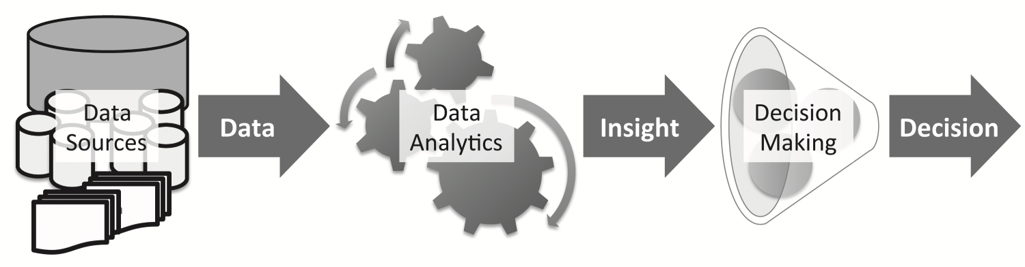
\includegraphics[width=0.8\linewidth,keepaspectratio]{predict}
\end{center}
\end{frame}

%%%%%%%%%%%%%%%%%%%%%%%%%%%%%%%%%%%%%%%%%%%%%%%%%%%%%%%%%%%
\begin{frame}[fragile]\frametitle{Applications}
\begin{itemize}
\item Businesses collect lots of data
	\begin{itemize}
	\item Purchase information 
	\item Web site browsing habits
	\item Social network data
	\end{itemize}

\item Goals
	\begin{itemize}
	\item Customer profiling,
	\item Targeted marketing,
	\item Fraud detection
	\end{itemize}
\end{itemize}
\end{frame}


%%%%%%%%%%%%%%%%%%%%%%%%%%%%%%%%%%%%%%%%%%%%%%%%%%%%%%%%%%%
\begin{frame}[fragile]\frametitle{Process}
\begin{center}
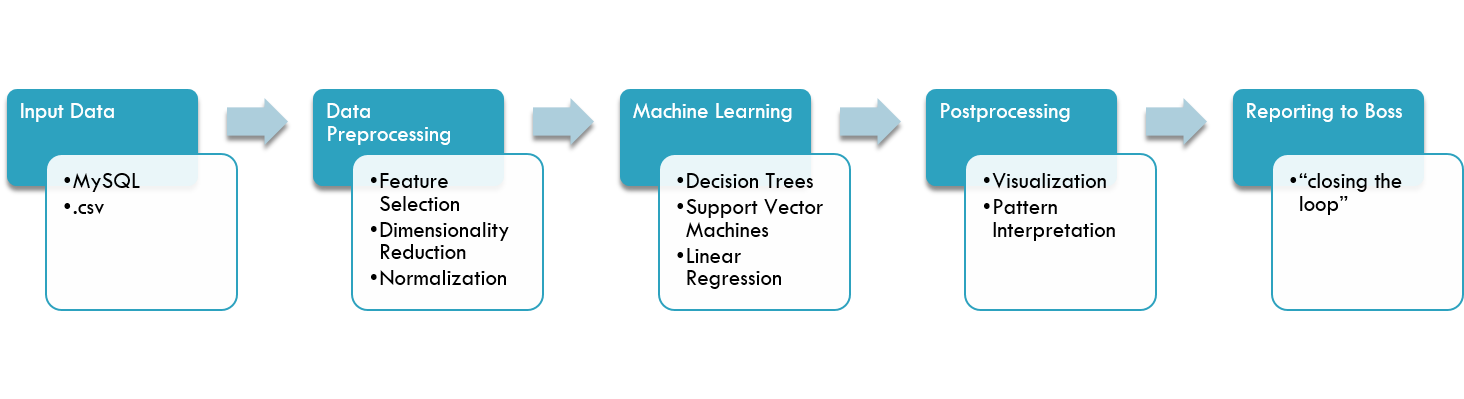
\includegraphics[width=0.8\linewidth,keepaspectratio]{process}
\end{center}
\end{frame}


%%%%%%%%%%%%%%%%%%%%%%%%%%%%%%%%%%%%%%%%%%%%%%%%%%%%%%%%%%%
\begin{frame}[fragile]\frametitle{Input Data}
\begin{itemize}
\item Available in data in variety of formats:
	\begin{itemize}
	\item Flat files (.csv or .txt)
	\item Spreadsheets (Excel .xls tougher to deal with)
	\item Relational tables (MySQL)
	\item Text, data on web page (scraping necessary)
	\end{itemize}
\item Big Data / Data Warehouse
\item Data spread out over multiple locations
\end{itemize}
\end{frame}


%%%%%%%%%%%%%%%%%%%%%%%%%%%%%%%%%%%%%%%%%%%%%%%%%%%%%%%%%%%
\begin{frame}[fragile]\frametitle{Preprocessing}
\begin{itemize}
\item To transform raw input data into an appropriate format for subsequent analysis:
	\begin{itemize}
	\item Fusing data from multiple sources
	\item Cleaning data to remove noise
	\item Duplicate observations
	\end{itemize}
\item Selecting records and features that are relevant to the data mining task at hand
\end{itemize}
\end{frame}

%%%%%%%%%%%%%%%%%%%%%%%%%%%%%%%%%%%%%%%%%%%%%%%%%%%%%%%%%%%
\begin{frame}[fragile]\frametitle{Machine Learning}
\begin{itemize}
\item Linear Regression
\item Support Vector Machines
\item Decision Trees
\item Clustering
\end{itemize}
\end{frame}


%%%%%%%%%%%%%%%%%%%%%%%%%%%%%%%%%%%%%%%%%%%%%%%%%%%%%%%%%%%
\begin{frame}[fragile]\frametitle{Postprocessing}
\begin{itemize}
\item Hypothesis testing to eliminate spurious data mining results
\item Statistical significant tests, confidence intervals, 
\item Visualization
\end{itemize}
\end{frame}


%%%%%%%%%%%%%%%%%%%%%%%%%%%%%%%%%%%%%%%%%%%%%%%%%%%%%%%%%%%
\begin{frame}[fragile]\frametitle{Challenges}
\begin{itemize}
\item Scalability
	\begin{itemize}
	\item Gigabytes, terabytes, petabytes, exabytes of data
	\item Storage capacity, streaming?
	\item Limits of python libraries
	\end{itemize}
\item Heterogeneous and Complex Data
\item High Dimensionality
	\begin{itemize}
	\item Datasets with hundreds or thousands of attributes
	\item Many variables are collected; few turn out to be useful
	\end{itemize}
\item Need to reduce data
	\begin{itemize}
	\item To avoid redundancy
	\item For effieciency: time, resources
	\end{itemize}
\end{itemize}
\end{frame}

%%%%%%%%%%%%%%%%%%%%%%%%%%%%%%%%%%%%%%%%%%%%%%%%%%%%%%%%%%%
\begin{frame}[fragile]\frametitle{What is Data Reduction?}
\begin{itemize}
\item Virtually all data analysis focuses on data reduction
\item Data reduction lets us see critical features or patterns in the data
\item Data reduction comes in the form of:
\begin{itemize}
\item Descriptive statistics
\item Measures of association
\item Graphical visualizations
\end{itemize}
\end{itemize}
\end{frame}


%%%%%%%%%%%%%%%%%%%%%%%%%%%%%%%%%%%%%%%%%%%%%%%%%%%%
\begin{frame}[fragile] \frametitle{Summary}

\adjustbox{valign=t}{
\begin{minipage}{0.45\linewidth}
Traditional Data Analysis
\begin{itemize}
%\item Hypothesis-and-test pattern
%\item Data collection
\item Laborious process
\item Generation and evaluation of thousands of hypotheses
\item Usually on relatively smaller datasets
\end{itemize}
\end{minipage}
}
\hfill
\adjustbox{valign=t}{
\begin{minipage}{0.45\linewidth}
Current Data Analysis
\begin{itemize}
\item Datasets analyzed typically not result of a carefully designed experiment

\item Datasets of size TB
\item Opportunistic data reduction
%\item Because of data quantity, role of traditional statistical concepts (confidence intervals, statistical significance tests) is reduced
%\item With large data sets, almost any small difference becomes significant
\end{itemize}
\end{minipage}
}

\end{frame}
